\documentclass{beamer}

\usepackage{ucs}
\usepackage[utf8x]{inputenc}
\usepackage[T1]{fontenc}
\usepackage[english]{babel}

\usepackage[retainorgcmds]{IEEEtrantools}%	IEEEeqnarray

\usepackage{mathabx}%	convolution symbol
\usepackage{multi row}
\usepackage{epstopdf}
\usepackage{listings}
\lstset{
	language=c,
	basicstyle=\footnotesize,
	showtabs=true,
	tabsize=3,
}

%	presentation info
\title{Projecto Integrado - Apresentação Intermédia 2}

\author{António Silva, Rui Brito}

\institute[pg22820, pg22781]{
	Universidade do Minho
}

\date{Braga, Março 2013}


%	beamer options
\usetheme{Frankfurt}


\begin{document}%	begin presentation

\maketitle%	title slide

\begin{frame}
	\frametitle{Índice}
	\tableofcontents
\end{frame}

\section{Modificações}
\begin{frame}
	\frametitle{Modificações na BD}

	\begin{figure}[!htp]
		\includegraphics[totalheight=1.2\textheight,angle=90]{../bd2.eps}		
		\end{figure}

\end{frame}

\section{Linguagem de Actividades}
\begin{frame}
	\frametitle{Linguagem de anotação para a descrição das Actividades}

	\begin{itemize}
		\item Modelado a partir da BD;
		\item Implementação em PHP;
		\begin{itemize}
			\item Reduzir complexidade;
			\item XSL implica gerar o SQL ou o próprio PHP;
		\end{itemize}
		\item DOMDocument e DOMXpath
	\end{itemize}

\end{frame}

\begin{frame}[fragile]
	\frametitle{Exemplo de XML}


\tiny
	\begin{verbatim}
<activities>
  <activities key="ex1">
    <begin_date>01/01/2012</begin_date>
    <end_date>31/12/2012</end_date>
    <description>Exemplo de uma actividade</description>
    <institution>
      <org type="Public University">
        <name>Universidade do Minho</name>
        <address>Gualtar</address>
        <country>Portugal</country>
      </org>
    </institution>
    <partners>
      <partner>J. J. Almeida</partner>
      <partner>Bruno Fernandes</partner>
    </partners>
    <conference is_organizator="false">
<name>JOIN - Jornadas de Informática da Universidade do Minho</name>
      <place>Universidade do Minho - Gualtar</place>
    </conference>
  </activities>
	\end{verbatim}
\normalsize

\end{frame}

\section{Descrição de Publicações}
\begin{frame}
	\frametitle{Formato Standard para a Descrição de Publicações}
	\begin{itemize}
		\item Módulo Perl (paradigma OO)
		\item Processa BibTeX 
		\item Organiza Informação por autor
		\item Insere por categoria na BD
		\item Ênfase em código genérico e facilmente extensível
	\end{itemize}
\end{frame}

\begin{frame}[fragile]
	\frametitle{Exemplo de Utilização}
\begin{verbatim} 
my $f = BibTeX::toDB->new(’bibtex.bib’,
	       ’DBI:mysql:database’,’user’,’pass’);

$f->parse("article");
$f->parse("techreport");
$f->parse("inproceedings");
$f->insertDB("J.J. Almeida");
\end{verbatim}
\end{frame}

\section{Interface Única}
\begin{frame}[fragile]
	\frametitle{Manifesto de um pacote gerado}
	\begin{verbatim}
		<cv> 
		  <info>
    <file>info.txt</file>
    <file>formation.txt</file>
  </info>
  <activities>
    <file>act.xml</file>
    <file>act2.xml</file>
  </activities>
  <publications>
    <file>pub.bib</file>
  </publications>
</cv>
	\end{verbatim}
\end{frame}

\begin{frame}
	\begin{center}
		\Huge\bfseries
		Demo
	\end{center}
\end{frame}

\section{Questões}
\begin{frame}
\titlepage
	\begin{center}
		\Huge\bfseries
		- ? -
	\end{center}
\end{frame}

\end{document}%	end presentation